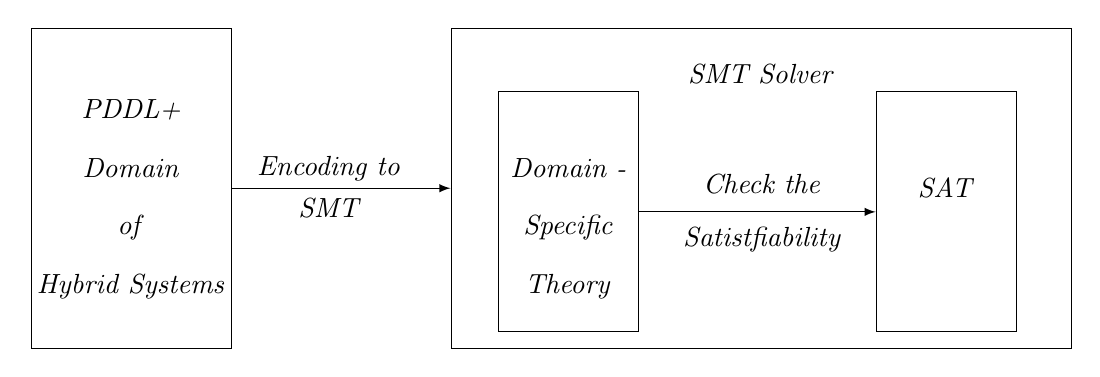
\begin{tikzpicture}[>=latex]
\begin{scope}

%   \draw  (1,1) rectangle (7,1.5);

%\filldraw[black] (0,0) circle (2pt) node[anchor=west] {s};
 
 
 \node[rectangle,draw,minimum width=1in, minimum height=1.6in] (p1) at (-6,0) {} ;
 
 \node (p1_d) at (-6,1) {\textit{PDDL+ }};
  \node (p1_d) at (-6,0.25) {\textit{Domain }};
   \node (p1_d) at (-6,-0.5) {\textit{of }};
    \node (p1_d) at (-6,-1.25) {\textit{Hybrid Systems }};
    
    \draw[->] (p1) edge (-1.95,0);
     \node (p1_d) at (-3.5,0.25) {$\textit{Encoding to}$};
     \node (p1_d) at (-3.5,-0.25) {$\textit{SMT}$};

\node[rectangle,draw,minimum width=3.1in, minimum height=1.6in] (p2) at (2,0) {} ;
 \node (p2_d) at (2,1.45) {\textit{SMT Solver }};
 

\node[rectangle,draw,minimum width=0.7in, minimum height=1.2in] (p3) at (-0.45,-0.3) {} ;
 \node (p3_d) at (-0.45,0.25) {\textit{Domain -}};
  \node (p3_d) at (-0.45,-0.5) {\textit{Specific }};
   \node (p3_d) at (-0.45,-1.25) {\textit{Theory }};
   
   \draw[->] (p3) edge (3.45,-0.3);
   \node (p3_d) at (2,0.05) {$\textit{Check the}$};
     \node (p3_d) at (2,-0.65) {$\textit{Satistfiability}$};

   
   
\node[rectangle,draw,minimum width=0.7in, minimum height=1.2in] (p4) at (4.35,-0.3) {} ;
 \node (p4_d) at (4.35,0) {\textit{SAT }};
   %\node (p4_d) at (4.35,-1.25) {\textit{Solver }};

  \end{scope}
\end{tikzpicture}